% !TEX encoding = UTF-8 Unicode
% author: josef dolezal
% git: https://github.com/josefdolezal
\documentclass[a4paper,11pt]{article}
\usepackage[czech]{babel}
\usepackage[utf8]{inputenc}
\usepackage[T1]{fontenc}
\usepackage{multirow}
\usepackage{hyperref}
\usepackage{listings}
\usepackage{algorithm}
\usepackage{graphicx}
\title{Sazba textu v \LaTeX}
\author{Josef Doležal}
\date{12. května 2015}

\begin{document}

	\maketitle

	\section{Řadící algoritmy}

	% blok převzatý z http://cs.wikipedia.org/wiki/Řadic%C3%AD_algoritmus
	% http://www.algoritmy.net/article/102/Asymptoticka-slozitost
	% http://sl.wikipedia.org/wiki/Mehurčno_urejanje
	Řadící algoritmus zajišťuje seřazení daného souboru dat do specifikovaného pořadí. Nejčastěji se řadí podle numerické velikosti čísel, případně abecedně. Řazení je velmi častá úloha, která je také částí mnoha dalších algoritmů; vývoji co možná nejefektivnějších algoritmů řazení se proto věnuje velké úsilí.
	
	Z hlediska řazení se vstupní data chápou jako soubor dvojic klíč--hodnota, přičemž po seřazení je posloupnost klíčů monotónní, zatímco na připojené hodnoty se při řazení nebere zřetel a pouze se přesouvají vždy s odpovídajícím klíčem. Při existenci několika položek se stejným klíčem se však podle pořadí odpovídajících hodnot rozlišují stabilní a nestabilní algoritmy.\cite{wiki}
	% konec bloku

	\subsection{Časová složitost}
	Složitost algoritmu udává, jak je daný algoritmus rychlý (kolik provede elementárních operací -- obrázek \ref{fig:img1}) vzhledem k množině vstupních dat. Ke klasifikaci algoritmů se obvykle používá tzv. asymtotická složitost, což je rozdělení algoritmů do tříd složitostí, u kterých platí, že od určité velikosti dat, je algoritmus dané třídy vždy pomalejší než algoritmus třídy předchozí, bez ohledu na to, jestli je některý z počítačů $c$-násobně výkonnější ($c$ je konstanta).

Škála v nekonečnu slouží k rozlišení jednotlivých tříd. Říká, že pokud se n\,blíží k nekonečnu, tak neexistuje reálná konstanta taková, aby byl algoritmus z vyšší třídy rychlejší než ten z třídy přechozí.\cite{algoritmy}
	
	$1<\log (n) < n < n \cdot \log (n) < n^k < k^n < n! < n^n$
	
	\begin{table}[H]\catcode`\-=12
		\centering
		\caption{Vybrané řadící algoritmy\cite{wiki}}
		\label{tab:tab1}
		\begin{tabular}{| l | l | l | l |} \hline
			\multirow{2}{*}{Název} & \multicolumn{3}{|c|}{Složitost} \\ \cline{2-4}
			 & Minimun & Průměr & Maximum \\ \hline
			Bubble sort & $O(n)$ & $O(n^2)$ & $O(n^2)$ \\ \hline
			Insertion sort & $O(n)$ & $O(n^2)$ & $O(n^2)$ \\ \hline
			Quicksort & $O(n^2)$ & $O(n \cdot \log n)$ & $O(n \cdot \log n)$ \\ \hline
			Selection sort & $O(n^2)$ & $O(n^2)$ & $O(n^2)$ \\ \hline
		\end{tabular}

	\end{table}
	
	\subsection{Běžné algoritmy}
	
	\begin{itemize}
		\item Bubble sort
		\item Heapsort
		\item Insertion sort
		\item Merge sort
		\item Quicksort
		\item Selection sort
	\end{itemize}
	
	\begin{figure}[H]
		\centering
    		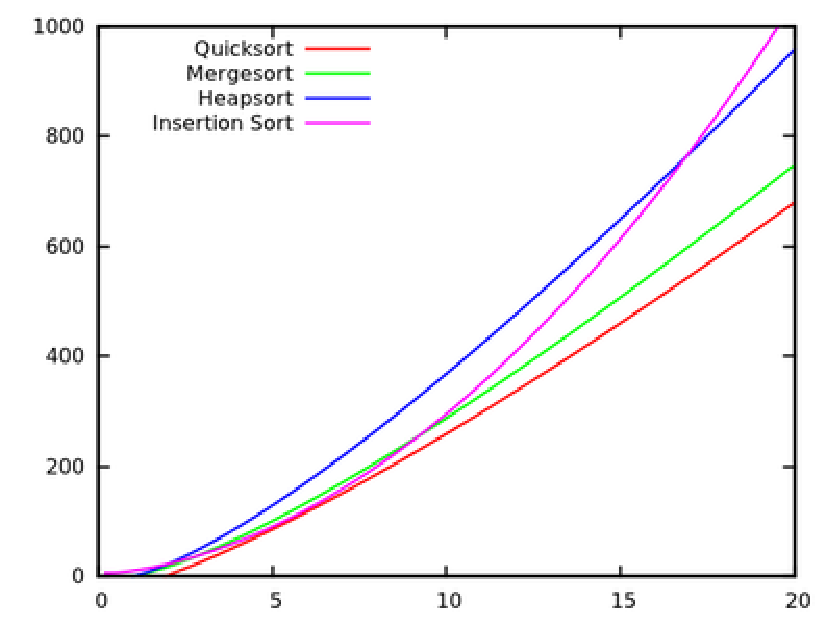
\includegraphics[width=0.7\textwidth,natwidth=400,natheight=300]{ilustrace2.pdf}
		\caption{Graf srovnání časové složitosti \cite{img1}}
		\label{fig:img1}
	\end{figure}
	
	\subsection{Bubble sort algoritmus}
	Bubble sort, česky také \uv{bublinkové} řazení, je implementačně jednoduchý řadicí algoritmus. Algoritmus opakovaně prochází seznam, přičemž porovnává každé dva sousedící prvky, a pokud nejsou ve správném pořadí, prohodí je. Pro praktické účely je neefektivní (tabulka \ref{tab:tab1}), využívá se hlavně pro výukové účely či v\,nenáročných aplikacích.
	
	\begin{algorithm}[H]
	\caption{Příklad implementace Bubble sortu v Javě}
	\begin{lstlisting}[language=java]
public static void bubbleSort(int[] array){
    for (int i = 0; i < array.length - 1; i++) {
        for (int j = 0; j < array.length - i - 1; j++) {
            if(array[j] < array[j+1]){
                int tmp = array[j];
                array[j] = array[j+1];
                array[j+1] = tmp;
            }
        }
    }
}
	\end{lstlisting}
	\end{algorithm}
	Cyklus tohoto algoritmu proběhne $(n-1) + (n-2) + (n-3) + (n-4) + \\ + (n-5) + (n-6) + ... + 1 = \frac{n \cdot ((n-1) + 1)}{2} = \frac{n^2}{2}$ krát (obrázek \ref{fig:img2}). Jeho asymptotická složitost je tedy $\Theta (n^2)$.\cite{algoritmy} Bubble je vysoce náročný na paměť počítače a může při svém běhu si může vyžádat $1\,\textup{kB}$ až desítky$\,\textup{MB}$.\cite{book}
	
	\begin{figure}[H]
		\centering
    		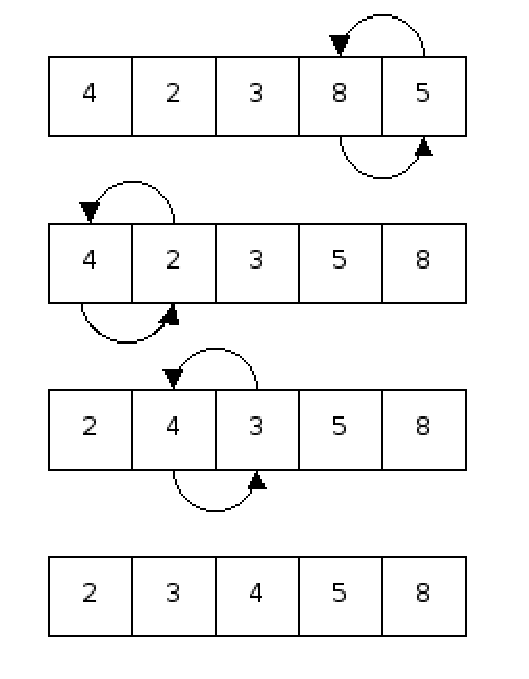
\includegraphics[width=0.3\textwidth,natwidth=254,natheight=326]{ilustrace1.pdf}
		\caption{Průběh řazení \cite{img2}}
		\label{fig:img2}
	\end{figure}
	
	\newpage
	
	\begin{thebibliography}{120}
		\bibitem{wiki}
		\textit{Wikipedie: otevřená encyklopedie, Řadící algoritmus} [online]. 
		[cit. {14.5.2015}],
		Dostupné z WWW:
		\url{http://cs.wikipedia.org/wiki/Řadic%C3%AD_algoritmus}
		
		\bibitem{algoritmy}
		\textit{Algoritmy.net - příručka vývojáře, Asymptotická složitost} [online]. 
		[cit. {14.5.2015}],
		Dostupné z WWW:
		\url{http://www.algoritmy.net/article/102/Asymptoticka-slozitost}
		
		\bibitem{book} Stephen G. Kochan.
		\textit{Objectiv-C 2.0}.
		Praha: Computer Press, 2010. 217 s. ISBN 987-80-251-2654-7.

		\bibitem{img1} 
		\textit{Graf srovnání časové náročnosti} [obrázek]. 
		\textit{sl.wikipedia.org} [online].
		[cit. {18.5.2015}],
		Dostupné z WWW:
		\url{http://sl.wikipedia.org/wiki/Mehurčno_urejanje}

		\bibitem{img2}
		\textit{Průběh řazení} [obrázek]. 
		\textit{cs.stackexchange.com} [online]. 
		[cit. {18.5.2015}],
		Dostupné z WWW:
		\url{http://cs.stackexchange.com/questions/3/why-is-quicksort-better-than-other-sorting-algorithms-in-practice}
		
	\end{thebibliography}
	
\end{document}






